\section{Przemek Orlikowski}
\label{sec:przorlik}


\begin{figure}[htbp] % Co oznacza [htbp]?
    \centering
    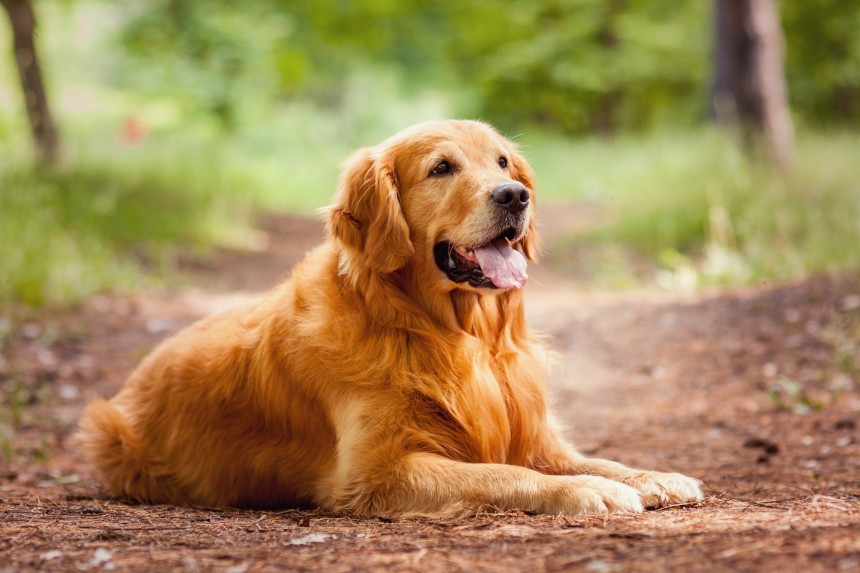
\includegraphics[width=0.4\textwidth]{pictures/pies-golden-retriever.jpg} % Jak sprawić, żeby obrazek był większy?
    \caption{This golden retriever is beautiful.}
    \label{fig:dog}
\end{figure}

\begin{itemize}
  \item Renegat
  \item Żółtodziób 
  \item Husky
\end{itemize}

\begin{enumerate}
  \item Rzym
  \item Sparta
  \item Ateny
\end{enumerate}



Tabela~\ref{tab:przemek}prezentuje przypadkowe daty. % Do czego służy \ref{}?
\begin{table}[]
\begin{tabular}{|l|l|l|l|l|}
\hline
\textbf{Rok} & \textbf{miesiac} & \textbf{dzien} & \textbf{godzina} & \textbf{minuta} \\ \hline
\textbf{1925}    & \textbf{10} & \textbf{27} & \textbf{9} & \textbf{8} \\ \hline
\textbf{1856}    & \textbf{12} & \textbf{18} & \textbf{10} & \textbf{5} \\ \hline
\textbf{1415}    & \textbf{9} & \textbf{11} & \textbf{6} & \textbf{13} \\ \hline
\end{tabular}

\label{tab:przemek}

\end{table}

\newpage


\textbf \textit{\Large{Armia Rzymu}} u szczytu potęgi liczyła ponad milion legionistów rozsianych po całym imperium. Armie o podonych liczbach wysstawiła dopiero napoleońska Francja na przełomie XVIII i XIX wieku. 
    
    \textbf Jako szczyt znaczenia liczebności sil na plu wlaki traktuje się XIX wiek oraz co warte podkreślenia I wojne światową. \textcolor{blue} {Miliony ofiar} po każdej ze stron na właściwie każdym froncie sprawiły. że dowódcy zaczęli szukać innych rozwiązań na polu walki.


A to ciekawe równanka:
$ x^{10} + y^{10} = z^9 $ \par
\begin{equation}
\begin{split}
I_Q = \sum_i \int \frac{dk}{2 \pi} \hbar \omega_i(k) v_i(k) \left[\frac{1}{e^{\hbar \omega_i(k) / (k_B T_h)} -1} - \frac{1}{e^{\hbar \omega_i(k) / (k_B T_c)} -1} \right] \\
\times T_{i}(\omega_i(k)) = \\
\sum_i \frac{\hbar}{2\pi} \int_{\omega_i^{min}}^{\omega_i^{max}} d\omega \omega T_{i}(\omega) 
\end{split}
\end{equation}
